%%%%%%%%%%%%%%%%%%%%%%%%%%%%%%%%%%%%%%%%%
% Beamer Presentation
% LaTeX Template
% Version 1.0 (10/11/12)
%
% This template has been downloaded from:
% http://www.LaTeXTemplates.com
%
% License:
% CC BY-NC-SA 3.0 (http://creativecommons.org/licenses/by-nc-sa/3.0/)
%
%%%%%%%%%%%%%%%%%%%%%%%%%%%%%%%%%%%%%%%%%

%----------------------------------------------------------------------------------------
%	PACKAGES AND THEMES
%----------------------------------------------------------------------------------------

\documentclass{beamer}

\mode<presentation> {

% The Beamer class comes with a number of default slide themes
% which change the colors and layouts of slides. Below this is a list
% of all the themes, uncomment each in turn to see what they look like.

%\usetheme{default}
%\usetheme{AnnArbor}
%\usetheme{Antibes}
%\usetheme{Bergen}
%\usetheme{Berkeley}
%\usetheme{Berlin}
%\usetheme{Boadilla}
%\usetheme{CambridgeUS}
%\usetheme{Copenhagen}
%\usetheme{Darmstadt}
%\usetheme{Dresden}
%\usetheme{Frankfurt}
%\usetheme{Goettingen}
%\usetheme{Hannover}
%\usetheme{Ilmenau}
%\usetheme{JuanLesPins}
%\usetheme{Luebeck}
\usetheme{Madrid}
%\usetheme{Malmoe}
%\usetheme{Marburg}
%\usetheme{Montpellier}
%\usetheme{PaloAlto}
%\usetheme{Pittsburgh}
%\usetheme{Rochester}
%\usetheme{Singapore}
%\usetheme{Szeged}
%\usetheme{Warsaw}

% As well as themes, the Beamer class has a number of color themes
% for any slide theme. Uncomment each of these in turn to see how it
% changes the colors of your current slide theme.

%\usecolortheme{albatross}
%\usecolortheme{beaver}
%\usecolortheme{beetle}
%\usecolortheme{crane}
%\usecolortheme{dolphin}
%\usecolortheme{dove}
%\usecolortheme{fly}
%\usecolortheme{lily}
%\usecolortheme{orchid}
%\usecolortheme{rose}
%\usecolortheme{seagull}
%\usecolortheme{seahorse}
%\usecolortheme{whale}
%\usecolortheme{wolverine}

%\setbeamertemplate{footline} % To remove the footer line in all slides uncomment this line
%\setbeamertemplate{footline}[page number] % To replace the footer line in all slides with a simple slide count uncomment this line

%\setbeamertemplate{navigation symbols}{} % To remove the navigation symbols from the bottom of all slides uncomment this line
}

\usepackage{graphicx} % Allows including images
\usepackage{booktabs} % Allows the use of \toprule, \midrule and \bottomrule in tables
\usepackage{multirow}
\usepackage{adjustbox}
\usepackage{array}
\newcommand{\xmark}{\textcolor{red}{\text{\sffamily X}}}
\newcommand{\cmark}{\textcolor{green}{\checkmark}}
\newcommand{\tr}{\text{tr}}
\newcommand{\E}{\textbf{E}}
\newcommand{\diag}{\text{diag}}
\newcommand{\argmax}{\text{argmax}}
\newcommand{\argmin}{\text{argmin}}
\newcommand{\Cov}{\text{Cov}}
\newcommand{\Vol}{\text{Vol}}

%----------------------------------------------------------------------------------------
%	TITLE PAGE
%----------------------------------------------------------------------------------------


\title[Informal]{How many neurons does it take to classify a lightbulb?}

\author{Charles Zheng} % Your name
\institute[Stanford] % Your institution as it will appear on the bottom of every slide, may be shorthand to save space
{Stanford University}
\date{\today} % Date, can be changed to a custom date

\begin{document}

\begin{frame}
\titlepage % Print the title page as the first slide
(Joint work with Yuval Benjamini)
\end{frame}

\begin{frame}
\frametitle{Overview}
\noindent\emph{Background and motivation}
\begin{itemize}
\item Information theory and network information theory
\item Entropy, conditional entropy, and mutual information
\item Studying the neural code
\item Functional fMRI study of face recognition
\end{itemize}
\noindent\emph{Questions}
\begin{itemize}
\item Can random stimuli samples be used to estimate mutual information?
\item Can we obtain mutual information from the Bayes error?
\item Can we obtain mutual information from observed classification rates?
\end{itemize}
\noindent\emph{Methods}
\begin{itemize}
\item Using Fano's inequality
\item Using low-SNR universality
\end{itemize}
\noindent\emph{Results}
\end{frame}

\section{Background}


\begin{frame}
\frametitle{Information theory} 
The complexity of modern communications system is made possible by Shannon's theory of information.
\begin{center}
\begin{tabular}{cc}
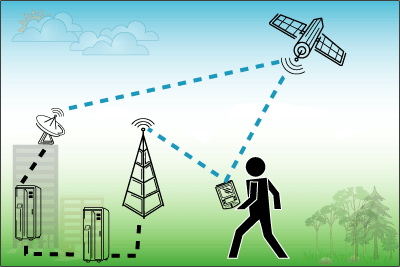
\includegraphics[scale =0.3]{communication-entry.png} &
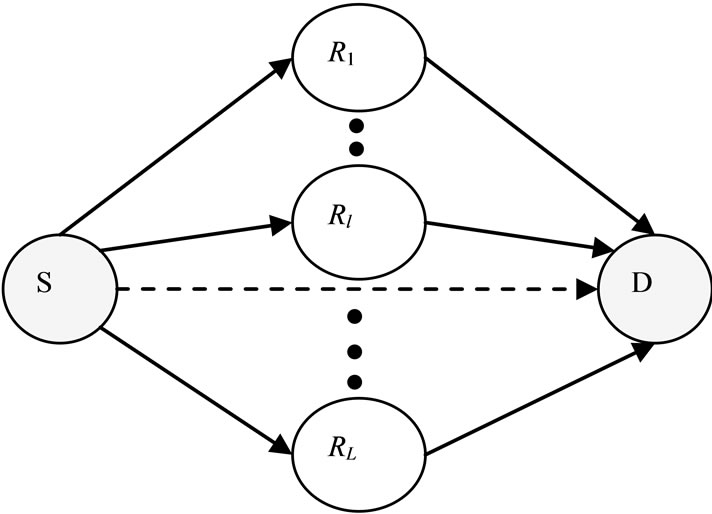
\includegraphics[scale =  0.2]{relay_channel.jpg}
\end{tabular}
\end{center}
A information-processing network can be analyzed in terms of interactions between its components (which are viewed as random variables.)
\note{ Modern communication systems depend
  on a vast network of signal transmitters and receivers.  All of this
  sophisticated engineering is made possible by information theory, a
  branch of applied mathematics introduced by Claude Shannon in 1948.
  Under the lens of information theory, we decompose a information
  network (e.g. the internet) into individual components (e.g. a
  server, a satellite) and view this collection of components as a
  collection of random variables, similar to a probabilistic graphical
  model.  Information theory defines quantities such as entropy,
  conditional entropy, and mutual information which serve to quantify
  how much information is contained in each component, and how the
  information is transmitted or lost as it passes through the network.
}
\tiny{Image credit CartouCHe, Aziz et al. 2011}
\end{frame}

\begin{frame}
\frametitle{Entropy and mutual information}
Let $X$ and $Y$ be real-valued random variables with a joint density $p(x, y)$ with respect to a measure $\mu$, and marginals $p_X(x)$ wrt $\mu_X$ and $p_Y(y)$ wrt $\mu_Y$.
The entropy, conditional entropy, and mutual information are nonlinear measures of spread, conditional spread, and dependence.

\vspace{0.5in}

\begin{tabular}{c|c|c}
\hline
Quantity & Definition & Linear analogue\\\hline
Entropy & $H(X) = - \int \log p(x) p(x) \mu_X(dx)$ & $\text{Var}(X)$\\
Conditional entropy & $H(X|Y) = \E[H(X|Y)]$ & $\E[\text{Var}(X|Y)]$\\
Mutual information & $I(X;Y) = H(X) - H(X|Y)$ & $\text{Cor}(X, Y)$\\\hline
\end{tabular}

\vspace{0.3in}

\small{The above definition includes both \emph{differential} entropy and \emph{discrete} entropy.
Information theorists tend to use log base 2, we will use natural logs in this talk.}
\end{frame}

\begin{frame}
\frametitle{Properties of mutual information}
\begin{center}
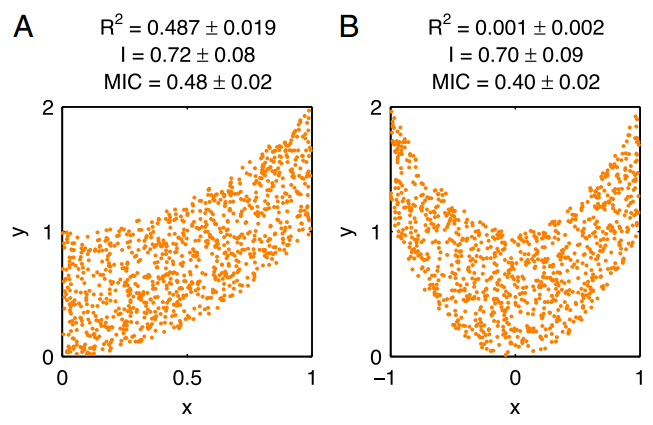
\includegraphics[scale = 0.2]{kinney.png}
\end{center}
\begin{itemize}
\item Nonnegative: $I(X;Y) \geq 0$
\item Symmetric: $I(X;Y) = I(Y; X)$
\item Bijection-invariant: $I(\phi(X); \psi(Y)) = I(\psi(Y);\phi(X)$.
\item Additivity.  If $(X_1,Y_1) \perp (X_2, Y_2)$, then
\[
I((X_1, X_2); (Y_1, Y2)) = I(X_1; Y_1) + I(X_2; Y_2)
\]
\item Relation to KL divergence $\mathbb{D}$.
\[
\mathbb{D}(p(x, y)||p(x)p(y)) = I(X; Y)
\]
\end{itemize}
\tiny{Image credit Kinney et al. 2014}
\end{frame}

\begin{frame}
\frametitle{Studying the neural code}
The brain is the \emph{most complex} information processing system we know!
\vspace{0.3in}
\begin{center}
\begin{tabular}{cc}
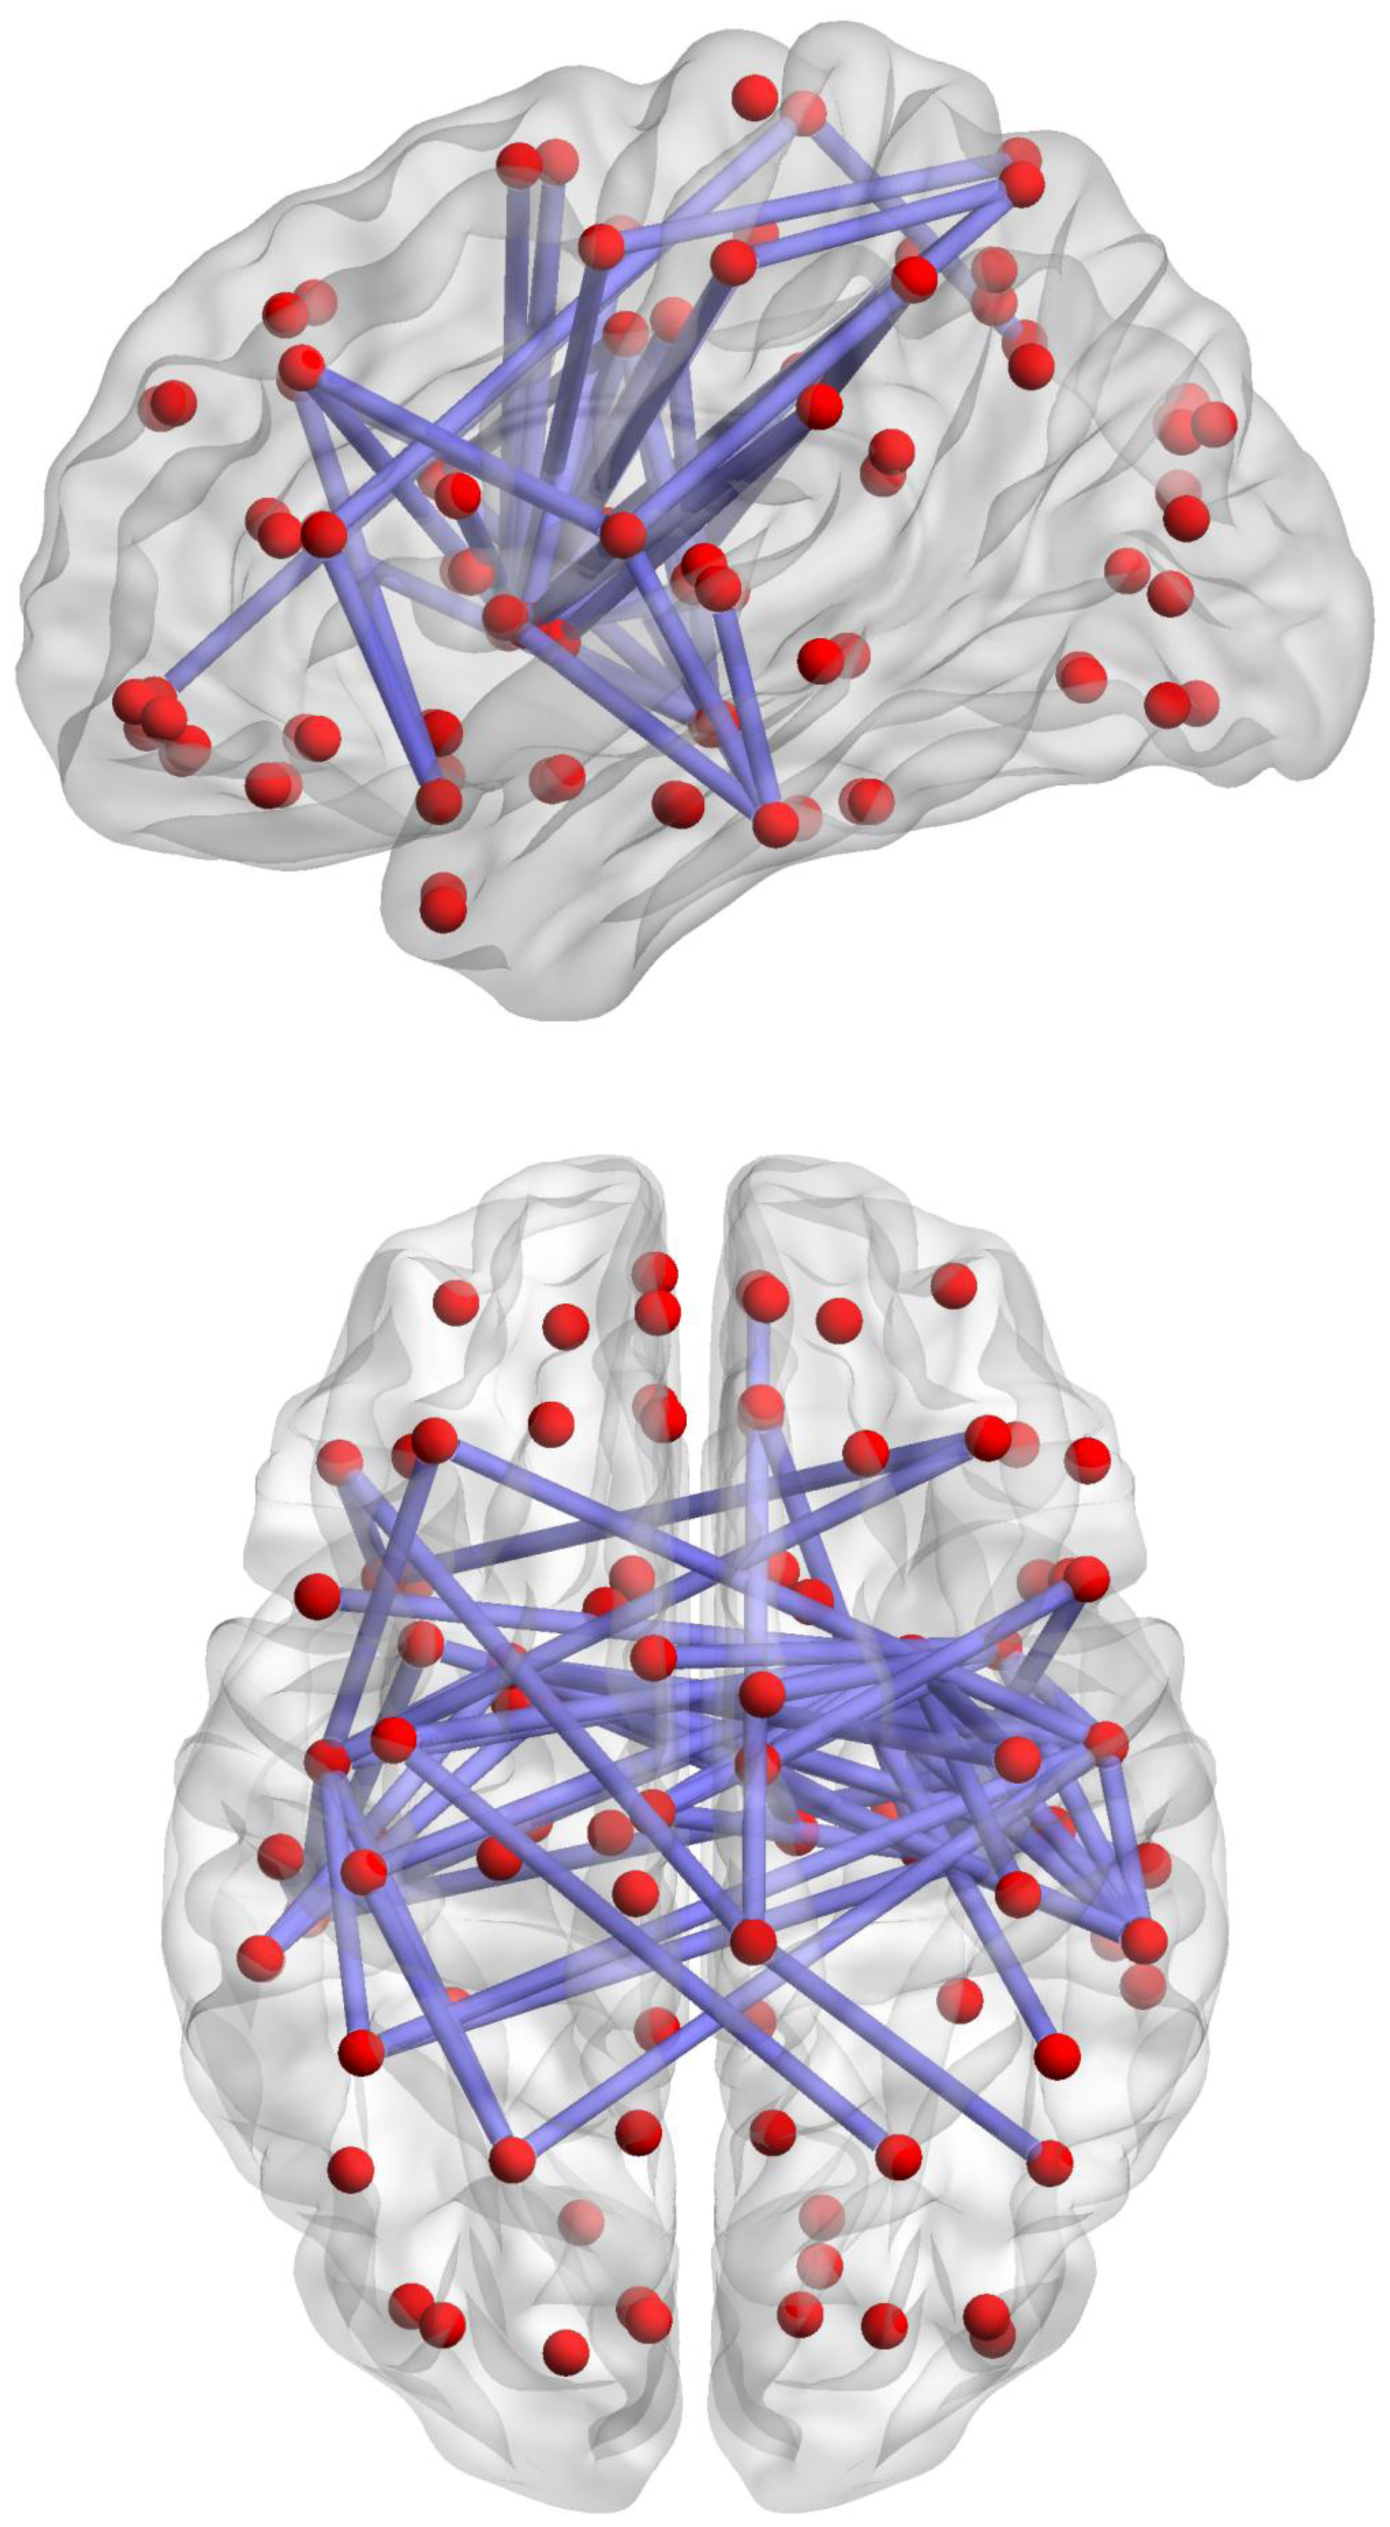
\includegraphics[scale = 0.3, clip =true, trim=0 0 0 2.5in]{Brain_network.png} &
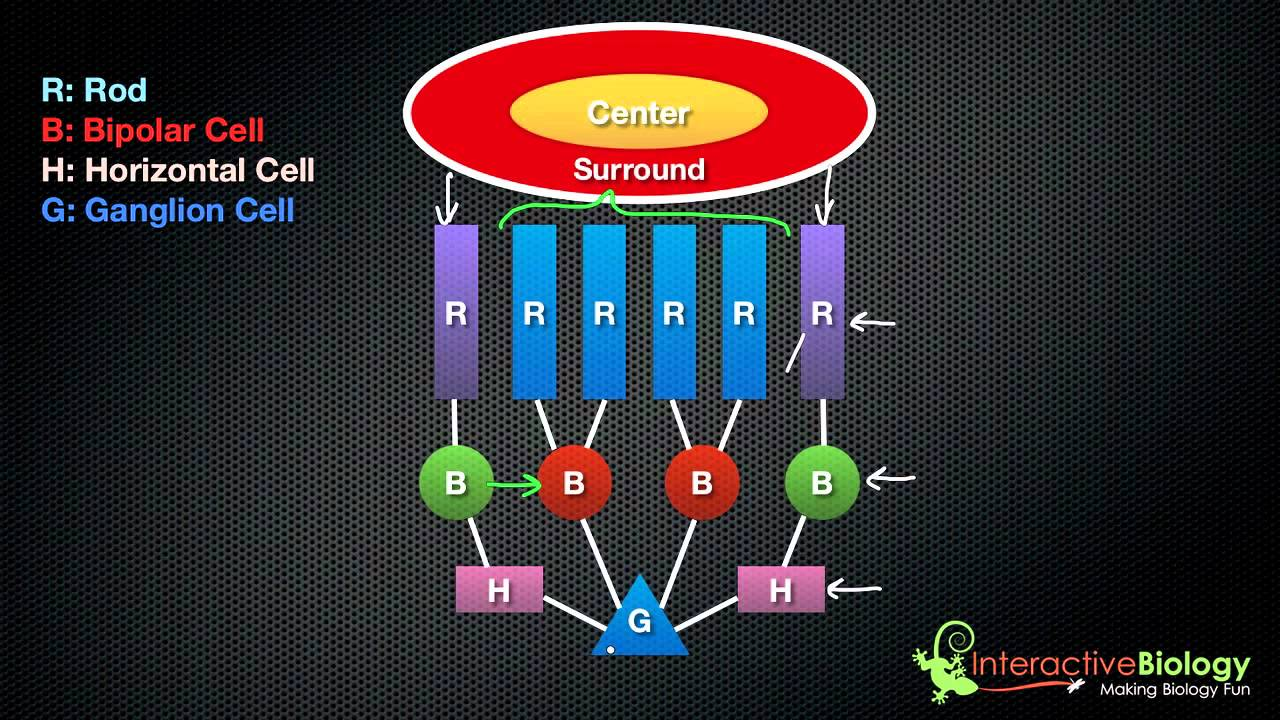
\includegraphics[scale = 0.1]{maxresdefault.jpg}\\
\small{Neural network inferred from data} & \small{Human retinal cells}\\
\small{(Hong et al.)} & 
\end{tabular}
\end{center}
\vspace{0.3in}
How do neurons encode, process, and decode sensory information?

\tiny{Image credit: Hong et al., Interactive Biology}
\end{frame}


\begin{frame}
\frametitle{References}
\begin{itemize}
\item Cover and Thomas.  Elements of information theory.
\item Muirhead.  Aspects of multivariate statistical theory.
\item van der Vaart.  Asymptotic statistics.
\end{itemize}
\end{frame}

\end{document}












